\chapter{Implementation}\label{ch:implement}
\todo[color=c05,inline]{testing the colors}

\section{Component Specifications}\label{ch:compSpec}
\todo[color=c05a,inline]{testing the colors}

\subsection{MOSFETs}
For the circuit the MOSFET C2M0160120D from Wolfspeed/Cree was chosen. 
It features a high blocking voltage, low on-resistance and low capacity.
That means it is able to work efficiently in high frequency power applications with small losses in switching, making it very suitable for converters.

The MOSFET is rated for switching voltages up to 1200V with a maximum current of 19A.
For switching a gate voltage of 14V is required and a negative input of -5V to -10V as a low input is recommended for fast switching.

\subsection{Diodes}
The used diode is the STTH6012 from STMicroelectronics.
The ultra fast soft recovery characteristics make it very efficient in high frequency pulse operation.
With a rating of 1200V repetitive peak reverse voltage and a maximum forward current of 60A the diode seems oversized but for experimental work they were used.

\subsection{Capacitors}
The chosen capacitors are standard sizes of $2.2 \mu F$ capacity with a voltage rating to 450V.

\subsection{Inductors}
%The inductor was winded by hand over a
\todo[color=c05a,inline]{missing}
\vspace{-8mm}
\section{Driver}\label{sec:driver}
\vspace{-3mm}
To control the MOSFETs the Semikron SKYPER 32R driver board has been chosen. \cite{Board1SK17:online} It can run two MOSFETs or IGBTs potential free with up to 1200V over the device.
It supports an output of +15V/-7V PWM with peak currents to 15A at frequencies up to 50kHz.
The board also comes with additional protection logic that was not used as failure detection and shut down input.
The input to the board are two PWM signals coming from the controller with Voltages of 0 to 15V.
To function the SKYPER board needs an external power supply of 15V,
some decoupling capacitors and capacitors to filter high frequency pulses.
These components are on the adaptor board also from Semikron.

On the secondary side of the board the two potential free PWM signals with -7 to 15V are given out.\cite{SKYPER322:online}
To adjust the switching properties of the device the output can be configured by changing the resistors $R_{on}$ and $R_{off}$.
They limit the current when switching in the state, so the device will switch slower.
Additionally external decoupling capacitors are needed. They are also on the adaptor board.
The failure detection logic was not used for testing.
A schematic of the secondary side of the SKYPER board can be seen in Figure \ref{fig:Skyper32out}.

\begin{figure}[H]
   \centering
   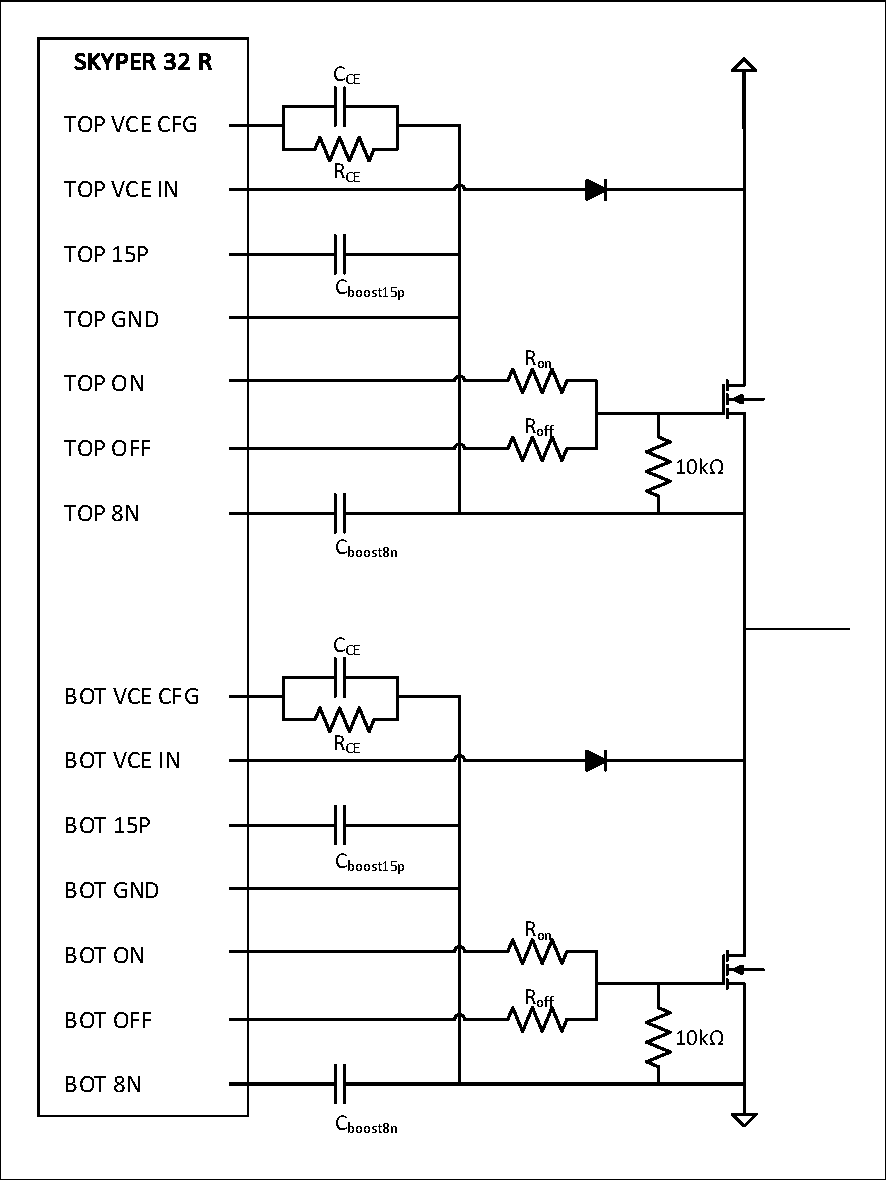
\includegraphics[width=0.5\textwidth]{figures/Skyperboard/Skyper32out.pdf}
    \caption{Circuit on the output of the SKYPER 32R}
	\label{fig:Skyper32out}
\end{figure}
\clearpage
As the SKYPER Board needs an input signal of 15V a circuit is needed to convert the 5V signal from the low power logic.
Therefore a small op-amp based comparator circuit was constructed.
It compares the input signal to 1.5 Volts, so every input above will result in a high output,
all inputs below as low.
This also allows to run it from a logic that only outputs 3V signals.

In Figure \ref{fig:Skyper32in} it can be seen how the input coming from the control logic with a 5V PWM signal and 15V power supply are connected to the amplification board.
On there the signal gets raised to 15V PWM and the board also includes the pull-up resistor to read out the open collector error out pin of the SKYPER 32R.
The board connects to the adaptor board that has the required capacitors and a pull up resistor for the error in.
The adaptor board is connected to all the inputs of the SKYPER 32R.

\begin{figure}[H]
   \centering
   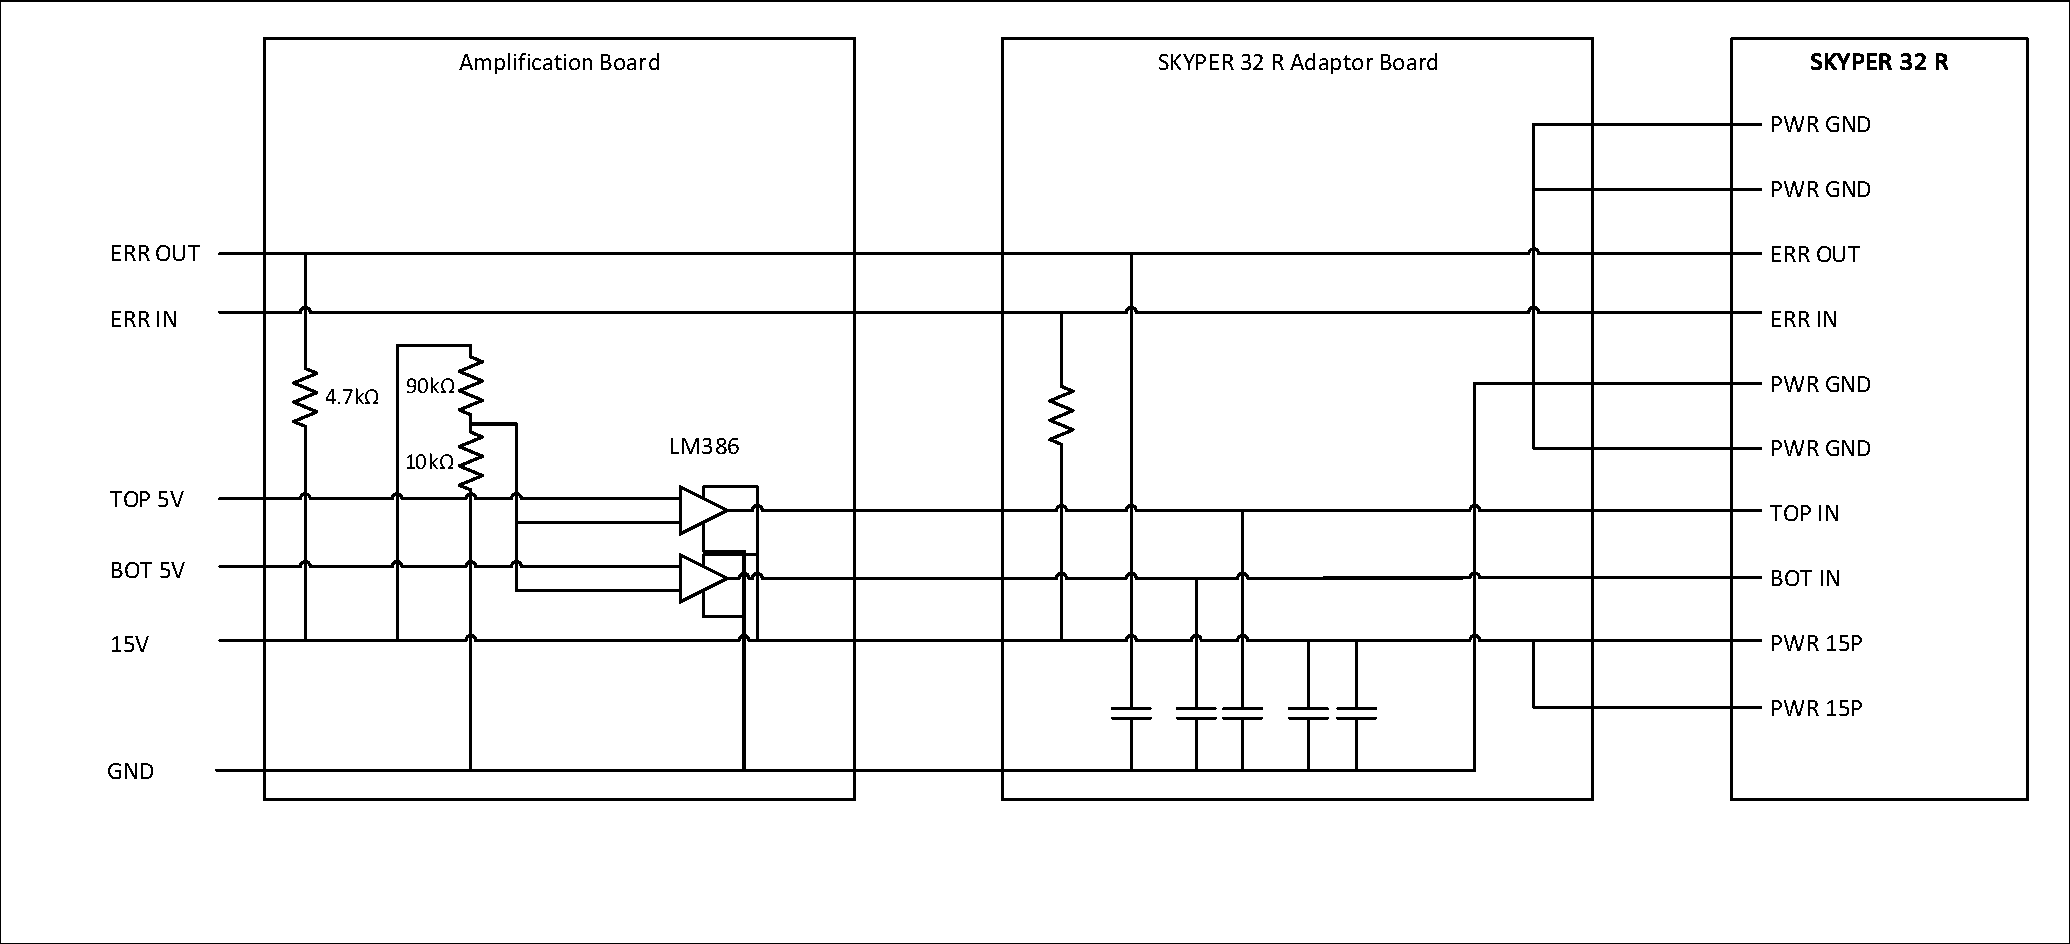
\includegraphics[width=\textwidth]{figures/Skyperboard/Skyper32in.pdf}
    \caption{Input boards for the SKYPER 32R}
	\label{fig:Skyper32in}
\end{figure}
The SKYPER board is intended for IGBT bridge circuits and therefore has a function which switches both devices off, if the input tries to turn them both on.\cite{SKYPER322:online} Therefore a second identical circuit and board will be used to drive each of the MOSFETs.

\clearpage
\section{PCB Design}\label{sec:PCB}

To be able to test the proposed topology,
a Printed Circuit Board (PCB) had to be made.
We started out designing a simple two stage layout,
and ended up manufacturing a three stage version.

\subsection{Two Stage PCB}
To get familiar with designing power electronics PCBs,
we started out designing a two stage version of the proposed topology.
Because we already had some familiarities with EAGLE from previous projects,
we used EAGLE for the first design attempts.
The finished design can be seen in Figure \ref{fig:2nxeagle}.

\begin{figure}[H]
	\begin{center}
	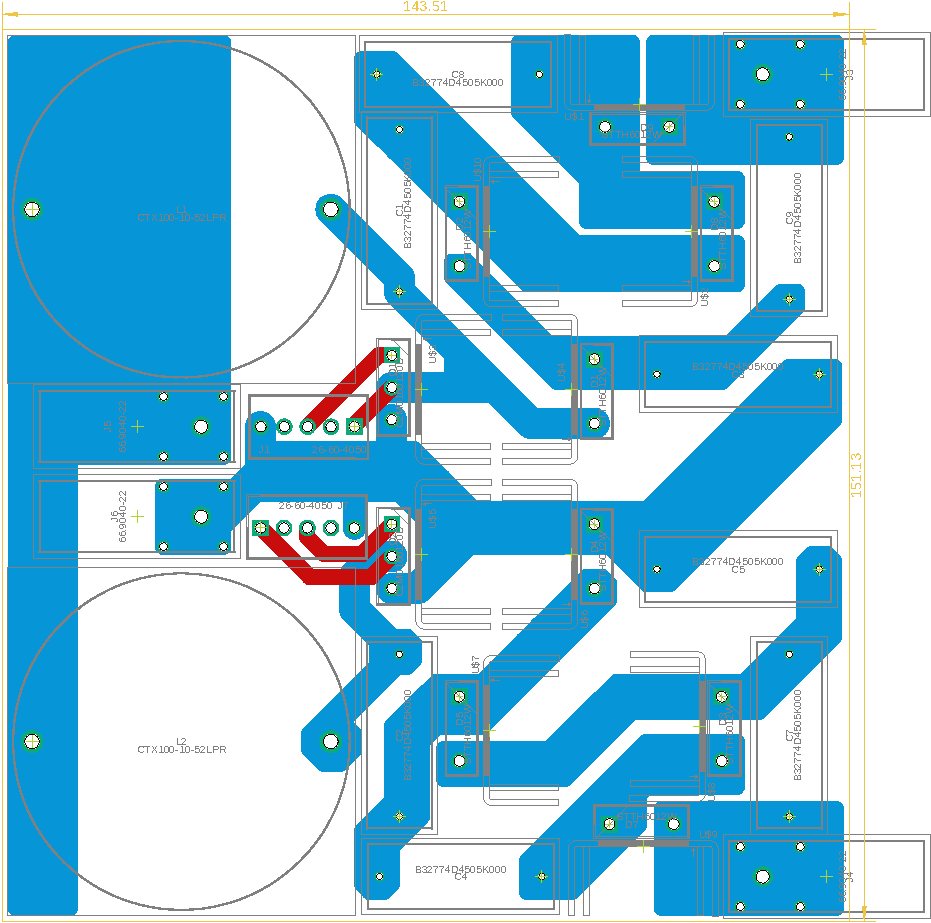
\includegraphics[width=0.6\textwidth]{figures/05cPCBdesign/2NX_interleaved_boost_converter_EAGLE_BY_DANIEL.pdf}
	\end{center}
	\caption{PCB Layout for a two stage 2NX Interleaved Boost Converter}
	\label{fig:2nxeagle}
\end{figure}

The red traces are logical signals,
located on the top layer of the PCB,
blue are power traces located on the bottom layer.
The power traces can be observed to be broader than the logic,
and were drawn as polygons,
to use the biggest available surface area.
The logical signals are designed to be as short as possible
and to be located as far from the power traces as possible,
to minimize interference.
\clearpage
Precautions were made in respect to the method of manufacturing,
because acute angles between two legs of a trace can lead to cracks in the trace when etching.
To prevent this from happening,
more copper was added in the areas in question to create obtuse angles.
A detailed view of this can be seen in Figure \ref{fig:2nxeagledetail}.
\begin{figure}[H]
	\begin{center}
	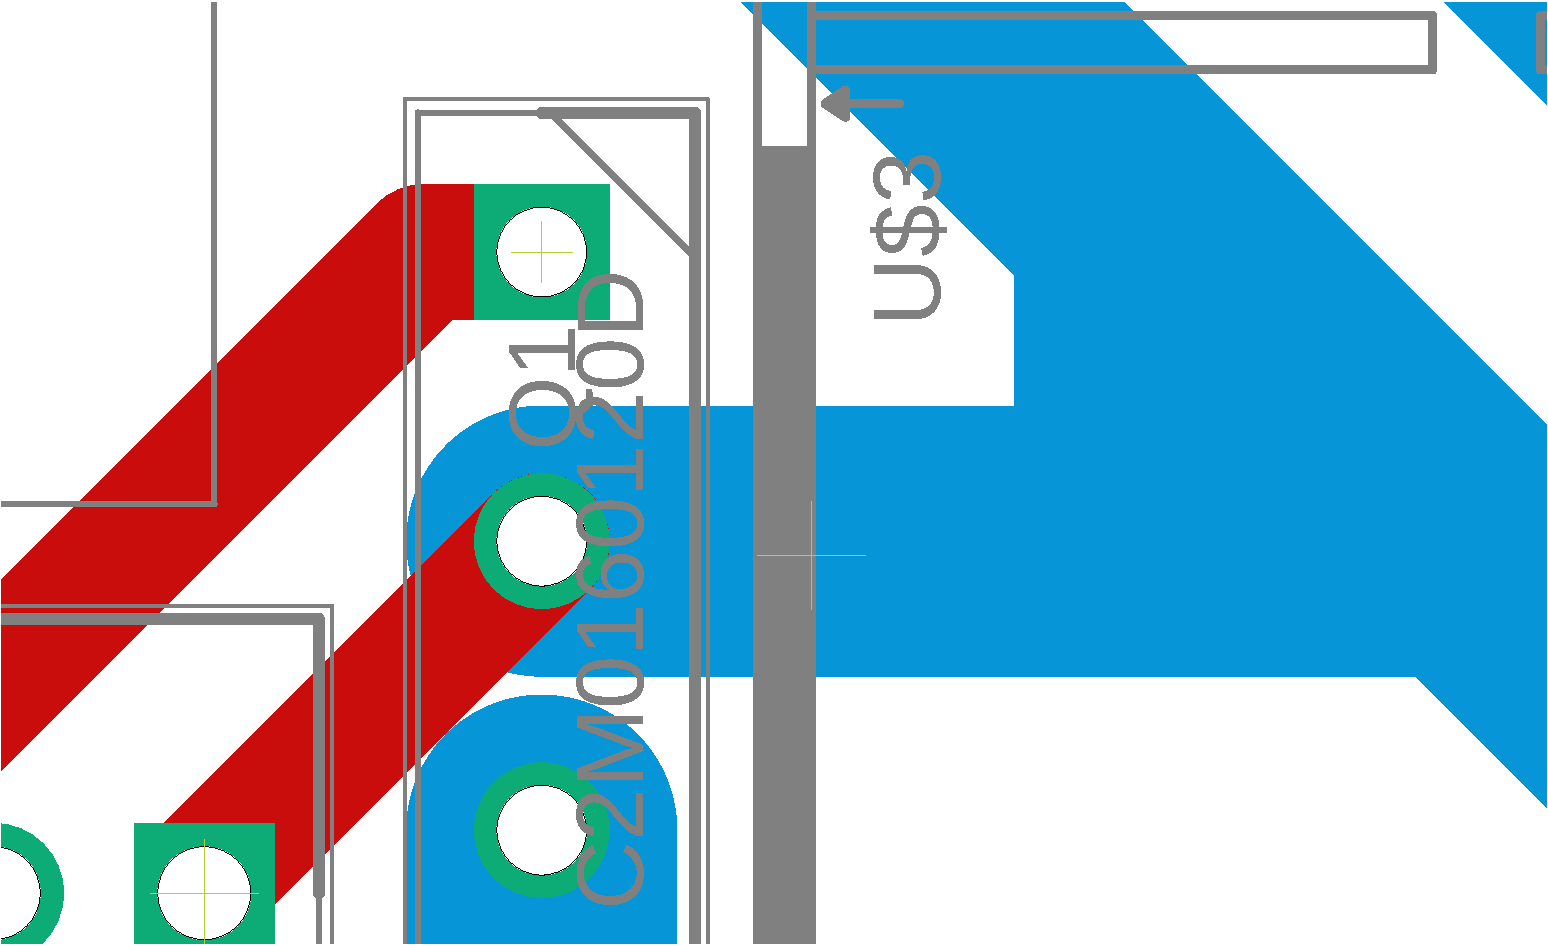
\includegraphics[width=0.6\textwidth]{figures/05cPCBdesign/2NX_interleaved_boost_converter_EAGLE_BY_DANIEL_DETAIL.pdf}
	\end{center}
	\caption{Detailed view of copper traces with obtuse angles}
	\label{fig:2nxeagledetail}
\end{figure}

\subsection{Three Stage PCB}\label{sub:3sPCB}
For the actual testing,
we decided on a three stage variant with our supervisor.
The PCB was again designed by us,
using feedback on the first design.
The power and logic traces are now on the same layer,
as it is not necessary to separate them as much.
The tracks generally are wider
and the spacing between is consistently kept at 2 mm.
The final PCB layout can be seen in Figure \ref{fig:multi2nxEAGLE}.

\begin{figure}[H]
	\begin{center}
	\includegraphics[height=1.0\textwidth,angle=270]{"figures/05cPCBdesign/FULL_3level_2NX_interleaved_boost_converter"}
	\end{center}
	\caption{PCB Layout for a multi stage 2NX Interleaved Boost Converter}
	\label{fig:multi2nxEAGLE}
\end{figure}
\vspace{+8mm}
The inductors and capacitors are different to the previous design,
because the new design reflects the components available to us.
To be able to connect the board to power and measurements,
banana plugs were suggested by our supervisor.

The inductor is not connected directly by soldering,
but through jumper cables.
This allows for easier access to the core and to fine tune the windings after testing.
This also makes measuring of voltage and current easier.

A detailed view showing the connectors for the top inductor can be seen in Figure \ref{fig:multi2nxDetail}.\\
The banana plugs for connecting the inductor are shown in red.

\begin{figure}[H]
	\begin{center}
	\includegraphics[width=0.5\textwidth]{"figures/05cPCBdesign/DETAiL_3level_2NX_interleaved_boost_converter"}
	\end{center}
	\caption{Detailed view of the inductor connection}
	\label{fig:multi2nxDetail}
\end{figure}

%
%\section{Static Modelling}\label{sec:statmod}
%
%\subsubsection{Single Pump Model}
%
%\begin{equation}
%	H = \bar{a_{2}} \cdot Q^2 + \bar{a_{1}} \cdot Q + \bar{a_{0}}
%	\label{eq:pumpHeadModel}
%\end{equation}
%\begin{equation}
%	P = \bar{b_{3}} \cdot Q^3 + \bar{b_{2}} \cdot Q^2 + \bar{b_{1}} \cdot Q + \bar{b_{0}}
%	\label{eq:pumpPowerModel}
%\end{equation}
%
%\begin{align*}
%	\left(\frac{\omega_1}{\omega_2}\right)^1 = \frac{Q_1}{Q_2} && 
%	\left(\frac{\omega_1}{\omega_2}\right)^2 = \frac{H_1}{H_2} &&
%	\left(\frac{\omega_1}{\omega_2}\right)^3 = \frac{P_1}{P_2}		
%\end{align*}\cite{Volk2014}.
%
%\begin{equation}
%	H(\omega) = a_0 \cdot \omega^2 + a_1 \cdot \omega \cdot Q(\omega) + a_2 \cdot Q(\omega)^2
%	\label{eq:pumpHeadModel2}
%\end{equation}
%\begin{equation}
%	P(\omega) = b_0 \cdot \omega^3 + b_1 \cdot \omega^2 \cdot Q(\omega) + b_2 \cdot \omega \cdot Q(\omega)^2 + b_3 \cdot Q(\omega)^3
%	\label{eq:pumpPowerModel2}
%\end{equation}
%
%\begin{align*}
%	a_0 = \frac{\bar{a_0}}{\bar{\omega_0^2}} && a_1 = \frac{\bar{a_1}}{\bar{\omega_0}} && a_2 = \bar{a_2} \\
%	b_0 = \frac{\bar{b_0}}{\bar{\omega_0^3}} && b_1 = \frac{\bar{b_1}}{\bar{\omega_0^2}} && b_2 = \frac{\bar{b_2}}{\omega_0} && b_3 = \bar{b_3}
%\end{align*}
%\cite{Yang2010}
%
%%\begin{figure}[ht]
%%	\centering
%%	\includegraphics[width=1\textwidth]{figures/05mathematicalModelling/flowVsPowerRun34.eps}
%%	\caption{Data Points for Flow vs. Power Consumption}
%%	\label{fig:flowVsPowerConsumption}
%%\end{figure}
%
%\begin{align*}
%	a_0 = -0.03044 && a_1 = 0.07635  && a_2 = 1.688  \\
%	b_0 = -0.2825 && b_1 = -0.7147 && b_2 = 54.39 && b_3 = 163.7 \\
%\end{align*}
%
%\section{Dynamic Modelling}\label{sec:dynMod}
%
%\begin{equation}
%	\frac{Y(s)}{U(s)} = \frac{A \cdot e^{-st_d}}{\tau \cdot s + 1}
%	\label{eq:plantTransferFunction}
%\end{equation}
%
%\begin{itemize}
%	\item A = final value the step response settles at
%	\item $t_{d}$ = time delay
%	\item $\tau$ = time it takes from 0.1 of final value to 0.9 final value
%\end{itemize}
